\subsection{Mismatched Crowdsourcing}
\label{s6:mc}

%\begin{figure}
%  \centerline{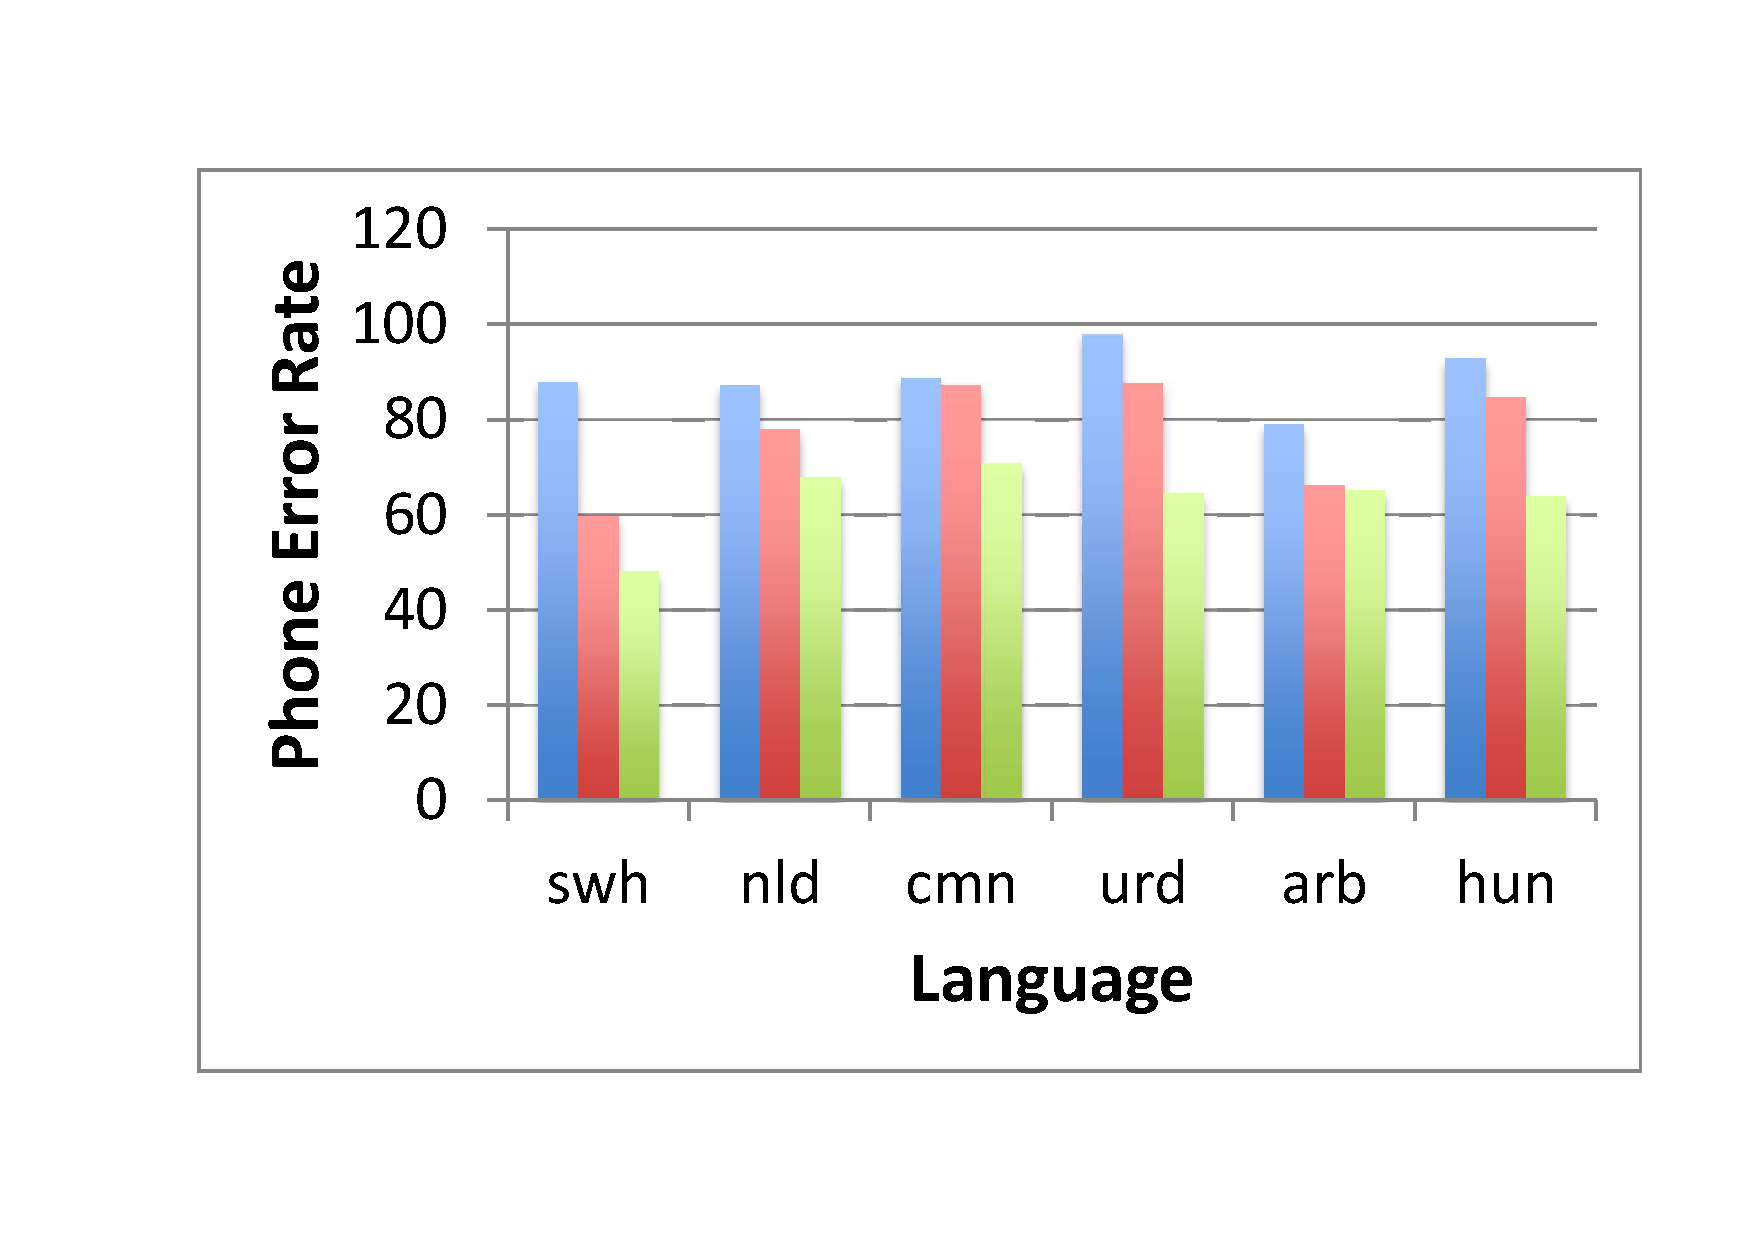
\includegraphics[width=0.7\columnwidth]{../figs/lm_results.pdf}}
%  \vspace*{-0.7cm}
%  \caption{LPER of the 1-best path: a measure of the quality of
%    probabilistic transcriptions acquired from mismatched
%    crowdsourcing.  Native transcriptions were available in six
%    languages: Swahili (swh), Dutch (nld), Mandarin (cmn), Urdu (urd),
%    Arabic (arb), and Hungarian (hun).  Probabilistic transcriptions
%    were decoded using three different methods per language: using a
%    universal phone set (leftmost bar in each language), using a
%    phone set specific to the target language (middle bar in each
%    language), and using a phonotactic language model derived from
%    Wikipedia texts (rightmost bar in each language).}
%  \label{fig:pt_decode_per}
%\end{figure}

The quality of a probabilistic transcription derived from mismatched
crowdsourcing is significantly improved by using a phone language
model during the decoding process ($\rho(\phi)$ in Eq.~(\ref{eq:PT})).
A crude measure of the quality of the PTs is given by the label phone error
rate (LPER), which measures the difference
between $\phi^* = \argmax_{\phi} \rho(\phi|T)$ and a native transcription. Phone
language models for each target language were computed from Wikipedia
texts using the methods described in Sec.~\ref{sec:trainwithlm}.
LPER of the 1-best path through the resulting PTs are shown in
Table.~\ref{tab:pt_decode_per}.  As shown, the use of a phonotactic
language model, derived from Wikipedia text, reduces PER by about 10\%
absolute, in each language.

\begin{table}
\centerline{\begin{tabular}{|c||c|c|c|c|c|}\hline
    Method & nld & cmn & urd & arb & hun \\\hline
    Universal set & 87.4 & 88.86 & 97.95 & 79.04 & 92.87 \\
    Target set & 78.12 & 87.4 & 87.81 & 66.39 & 84.78 \\
    Phone bigram & 68.0 & 70.88 & 64.67 & 65.29 & 63.98 \\\hline
\end{tabular}}
\vspace*{1mm}
\caption{Label phone error rate (LPER) of probabilistic transcriptions
  for nld=Dutch, cmn=Mandarin, urd=Urdu, arb=Arabic, hun=Hungarian.
  Methods: universal phone set, target-language phone set, text-based
  phone bigram.}
\label{tab:pt_decode_per}
\end{table}

%\begin{table}[t]
%\centering
%\begin{tabular}{|c||c|c|c|c|c|c|c|}
%  \hline
%  & \multicolumn{7}{|c|}{Language (ISO 639-3 Code)}\\ \hline
%& arb & yue & nld & hun & cmn & swh & urd \\ \hline\hline
%Dev set (1-best PER) & 65.8 & 66.4 & 68.9 & 63.7 & 70.9 & 47.6 & 67.2 \\
%Eval set (1-best PER) & 66.2 & 67.8 & 70.9 & 63.5 & 69.6 & 50.3 & 70.5 \\\hlineswh	88.05	59.78	48.08

%\end{tabular}
%\caption{Error rates (PER) of probabilistic transcripts computed from
%  mismatched crowdsourcing (non-native human listeners): Phone error
%  rate (PER) of the 1-best path through the probabilistic
%  transcription, $\phi^*=\argmax\rho(\phi|T)$, development and
%  evaluation sets.}
%\label{tab:LPER}
%\end{table}

%Table~\ref{tab:LPER} lists LPERs on the development and evaluation
%sets, for all seven languages.
LPER of the 1-best path does not
accurately reflect the extent of information in the PTs that can be
leveraged during ASR adaptation.  Consider, for example, the four
Urdu phones~\ipa{[p,p\textsuperscript{h},b,\"*b]}.  An attentive
English-speaking transcriber must choose between the two letters
$<$p,b$>$ in order to represent any of these four phones.  The
misperception G2P therefore maps the letters $<$p,b$>$ into a
distribution over the phones~\ipa{[p,p\textsuperscript{h},b,\"*b]}.
There is no reason to expect that the maximizer of
$\rho(\phi|\lambda)$ is correct, but there is good reason to expect
the correct answer to be a member of a short $N$-best list ($N\le 4$
phones/grapheme).  A fuller picture is therefore obtained by
considering a collection of sequences $\phi$ that are almost as
probable as $\phi^*$ according to our model. Figure~\ref{fig:listPER}
shows the trend of phone error rates (for three languages) obtained by
using collections $\phi$ of increasing size, plotted against an
entropy estimate of $\phi$, e.g., 1 bit of entropy allows two equally
probable choices for each phone in $\phi$. We note that the phone
error rates significantly drop across all languages, staying within 1
bit of entropy per phone, illustrating the extent of information
captured by the PTs.

\begin{figure}[t!]
  %\centerline{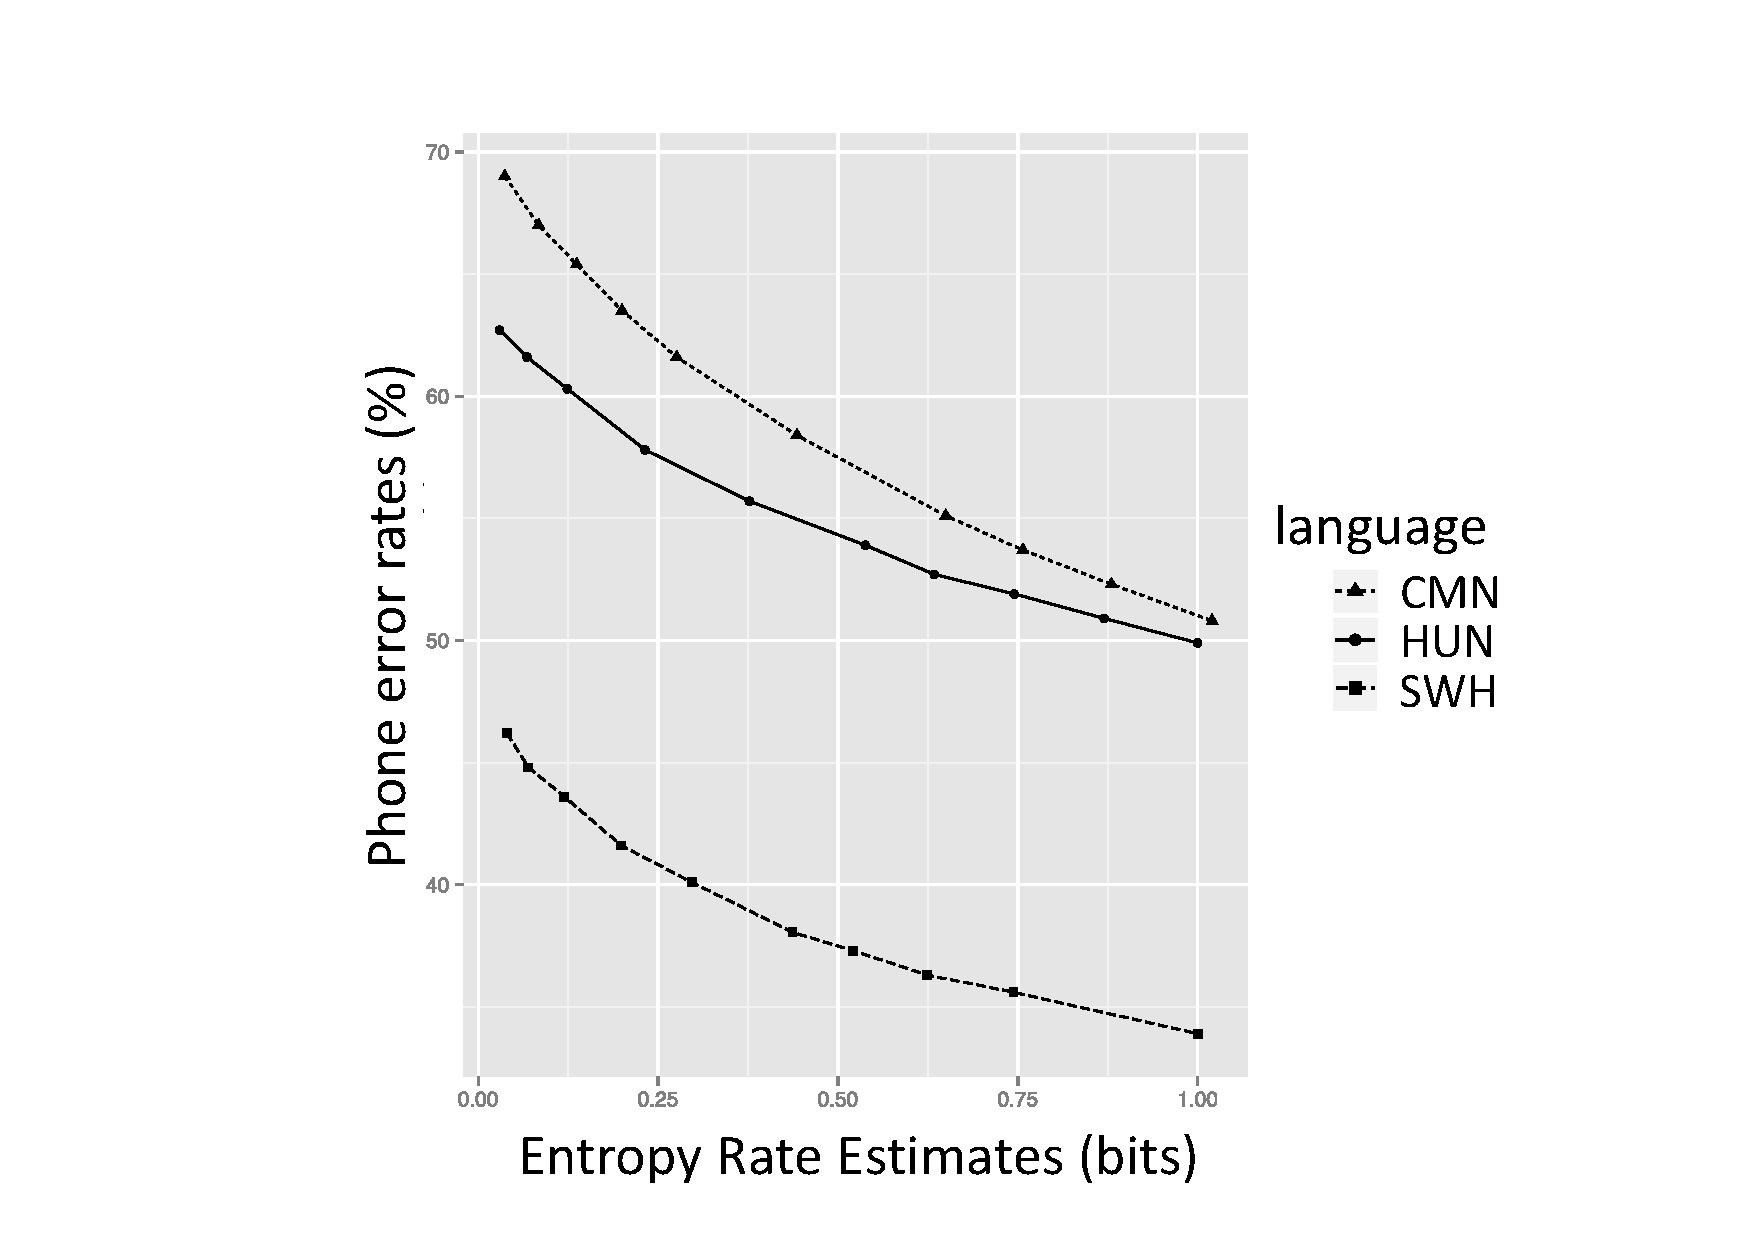
\includegraphics[width=0.7\columnwidth]{../figs/ptperfigure.pdf}}
  \begin{center}
\begin{tikzpicture}[
    scale=\mytikzscale,
    every node/.style={transform shape}]
\draw[<->] (0,-0.5) to (0,4.5);
\draw[<->] (-0.5,0) to (10.5,0);
\draw (-0.1,0.5) to (0.1,0.5);
\node at (-0.25,0.5) {35};
\draw (-0.1,1.0) to (0.1,1.0);
\node at (-0.25,1.0) {40};
\draw (-0.1,1.5) to (0.1,1.5);
\node at (-0.25,1.5) {45};
\draw (-0.1,2.0) to (0.1,2.0);
\node at (-0.25,2.0) {50};
\draw (-0.1,2.5) to (0.1,2.5);
\node at (-0.25,2.5) {55};
\draw (-0.1,3.0) to (0.1,3.0);
\node at (-0.25,3.0) {60};
\draw (-0.1,3.5) to (0.1,3.5);
\node at (-0.25,3.5) {65};
\draw (-0.1,4.0) to (0.1,4.0);
\node at (-0.25,4.0) {70};
\draw (1,-0.1) to (1,0.1);
\node at (1,-0.25) {0.1};
\draw (2,-0.1) to (2,0.1);
\node at (2,-0.25) {0.2};
\draw (3,-0.1) to (3,0.1);
\node at (3,-0.25) {0.3};
\draw (4,-0.1) to (4,0.1);
\node at (4,-0.25) {0.4};
\draw (5,-0.1) to (5,0.1);
\node at (5,-0.25) {0.5};
\draw (6,-0.1) to (6,0.1);
\node at (6,-0.25) {0.6};
\draw (7,-0.1) to (7,0.1);
\node at (7,-0.25) {0.7};
\draw (8,-0.1) to (8,0.1);
\node at (8,-0.25) {0.8};
\draw (9,-0.1) to (9,0.1);
\node at (9,-0.25) {0.9};
\node at (-1,2) {LPER};
\node at (5,-0.75) {Entropy of the PT (bits per segment)};
\node[rectangle,draw=black] at (12.5,2) {\begin{tabular}{l}-s- = Swahili\\-c- = Mandarin\\-h- = Hungarian\end{tabular}};
\node at (0.4,1.6200000000000003) {s};
\node at (0.37,3.9) {c};
\node at (0.3,3.2700000000000005) {h};
\node at (0.7000000000000001,1.4799999999999998) {s};
\node at (0.8400000000000001,3.7) {c};
\node at (0.68,3.16) {h};
\node at (1.2,1.36) {s};
\node at (1.37,3.5400000000000005) {c};
\node at (1.24,3.03) {h};
\node at (1.9900000000000002,1.1600000000000001) {s};
\node at (2.0,3.35) {c};
\node at (2.3200000000000003,2.78) {h};
\node at (2.9699999999999998,1.0100000000000002) {s};
\node at (2.7600000000000002,3.16) {c};
\node at (3.77,2.5700000000000003) {h};
\node at (4.37,0.8100000000000002) {s};
\node at (4.43,2.84) {c};
\node at (5.380000000000001,2.3899999999999997) {h};
\node at (5.21,0.7299999999999998) {s};
\node at (6.5,2.5100000000000002) {c};
\node at (6.34,2.2700000000000005) {h};
\node at (6.24,0.6299999999999997) {s};
\node at (7.57,2.37) {c};
\node at (7.45,2.19) {h};
\node at (7.4399999999999995,0.5600000000000002) {s};
\node at (8.8,2.2299999999999995) {c};
\node at (8.7,2.09) {h};
\node at (10.0,0.38999999999999985) {s};
\node at (10.2,2.0799999999999996) {c};
\node at (10.0,1.9899999999999998) {h};
\draw (0.4,1.6200000000000003) to (0.7000000000000001,1.4799999999999998);
\draw (0.7000000000000001,1.4799999999999998) to (1.2,1.36);
\draw (1.2,1.36) to (1.9900000000000002,1.1600000000000001);
\draw (1.9900000000000002,1.1600000000000001) to (2.9699999999999998,1.0100000000000002);
\draw (2.9699999999999998,1.0100000000000002) to (4.37,0.8100000000000002);
\draw (4.37,0.8100000000000002) to (5.21,0.7299999999999998);
\draw (5.21,0.7299999999999998) to (6.24,0.6299999999999997);
\draw (6.24,0.6299999999999997) to (7.4399999999999995,0.5600000000000002);
\draw (7.4399999999999995,0.5600000000000002) to (10.0,0.38999999999999985);
\draw (0.37,3.9) to (0.8400000000000001,3.7);
\draw (0.8400000000000001,3.7) to (1.37,3.5400000000000005);
\draw (1.37,3.5400000000000005) to (2.0,3.35);
\draw (2.0,3.35) to (2.7600000000000002,3.16);
\draw (2.7600000000000002,3.16) to (4.43,2.84);
\draw (4.43,2.84) to (6.5,2.5100000000000002);
\draw (6.5,2.5100000000000002) to (7.57,2.37);
\draw (7.57,2.37) to (8.8,2.2299999999999995);
\draw (8.8,2.2299999999999995) to (10.2,2.0799999999999996);
\draw (0.3,3.2700000000000005) to (0.68,3.16);
\draw (0.68,3.16) to (1.24,3.03);
\draw (1.24,3.03) to (2.3200000000000003,2.78);
\draw (2.3200000000000003,2.78) to (3.77,2.5700000000000003);
\draw (3.77,2.5700000000000003) to (5.380000000000001,2.3899999999999997);
\draw (5.380000000000001,2.3899999999999997) to (6.34,2.2700000000000005);
\draw (6.34,2.2700000000000005) to (7.45,2.19);
\draw (7.45,2.19) to (8.7,2.09);
\draw (8.7,2.09) to (10.0,1.9899999999999998);
  \end{tikzpicture}
\end{center}

  \vspace*{-1cm}
  \caption{LPER plotted against entropy rate estimates of phone sequences in three different languages.}
\label{fig:listPER}
\end{figure}

